%%%%%%%%%%%%%%%%%%%%%%%%%%%%%%%%%%%%%%%%%
% Beamer Presentation
% LaTeX Template
% Version 1.0 (10/11/12)
%
% This template has been downloaded from:
% http://www.LaTeXTemplates.com
%
% License:
% CC BY-NC-SA 3.0 (http://creativecommons.org/licenses/by-nc-sa/3.0/)
%
%%%%%%%%%%%%%%%%%%%%%%%%%%%%%%%%%%%%%%%%%

%----------------------------------------------------------------------------------------
%	PACKAGES AND THEMES
%----------------------------------------------------------------------------------------

\documentclass{beamer}

\mode<presentation> {

% The Beamer class comes with a number of default slide themes
% which change the colors and layouts of slides. Below this is a list
% of all the themes, uncomment each in turn to see what they look like.

%\usetheme{default}
%\usetheme{AnnArbor}
%\usetheme{Antibes}
%\usetheme{Bergen}
%\usetheme{Berkeley}
%\usetheme{Berlin}
%\usetheme{Boadilla}
%\usetheme{CambridgeUS}
%\usetheme{Copenhagen}
%\usetheme{Darmstadt}
%\usetheme{Dresden}
%\usetheme{Frankfurt}
%\usetheme{Goettingen}
%\usetheme{Hannover}
%\usetheme{Ilmenau}
%\usetheme{JuanLesPins}
%\usetheme{Luebeck}
\usetheme{Madrid}
%\usetheme{Malmoe}
%\usetheme{Marburg}
%\usetheme{Montpellier}
%\usetheme{PaloAlto}
%\usetheme{Pittsburgh}
%\usetheme{Rochester}
%\usetheme{Singapore}
%\usetheme{Szeged}
%\usetheme{Warsaw}

% As well as themes, the Beamer class has a number of color themes
% for any slide theme. Uncomment each of these in turn to see how it
% changes the colors of your current slide theme.

%\usecolortheme{albatross}
%\usecolortheme{beaver}
%\usecolortheme{beetle}
%\usecolortheme{crane}
%\usecolortheme{dolphin}
%\usecolortheme{dove}
%\usecolortheme{fly}
%\usecolortheme{lily}
%\usecolortheme{orchid}
%\usecolortheme{rose}
%\usecolortheme{seagull}
%\usecolortheme{seahorse}
%\usecolortheme{whale}
%\usecolortheme{wolverine}

%\setbeamertemplate{footline} % To remove the footer line in all slides uncomment this line
%\setbeamertemplate{footline}[page number] % To replace the footer line in all slides with a simple slide count uncomment this line

%\setbeamertemplate{navigation symbols}{} % To remove the navigation symbols from the bottom of all slides uncomment this line
}

\usepackage{graphicx} % Allows including images
\usepackage{booktabs} % Allows the use of \toprule, \midrule and \bottomrule in tables
\usepackage{times}
\usepackage{latexsym}
\usepackage{graphicx}
\usepackage{amsmath}
\usepackage{arydshln}
\usepackage{url}
\usepackage{color}
\usepackage{verbatim}
\usepackage{algorithm}
\usepackage{todonotes}
\usepackage{enumitem}
\usepackage{textcomp}
\usepackage{caption}
\captionsetup[figure]{labelformat=empty}
\usepackage{adjustbox}
\usepackage[noend]{algpseudocode}
\setbeamertemplate{caption}[numbered]
\newcommand{\softmax}{\mathrm{softmax}}
\DeclareMathOperator*{\argmax}{arg\,max}
\usepackage{bibentry}
\usetheme{Boadilla}
\usepackage{natbib}
%----------------------------------------------------------------------------------------
%	TITLE PAGE
%----------------------------------------------------------------------------------------
\usepackage{algpseudocode}
%\usepackage[style=ieee]{biblatex}
%\addbibresource{acl.bib}


\title[]{Language Model-Friendly Paraphrase Search} % The short title appears at the bottom of every slide, the full title is only on the title page

\author{Saeed Najafi (snajafi@ualberta.ca)}
% Your name
\institute[] % Your institution as it will appear on the bottom of every slide, may be shorthand to save space
{
%\small{Advised by Alona Fyshe (alona@ualberta.ca)}\\
%\small{Computing Science Department}\\
%\small{University of Alberta}
}
\date{\today}
% Date, can be changed to a custom date
\begin{document}
\setbeamertemplate{itemize items}[square]


\begin{frame}
\titlepage % Print the title page as the first slide
\end{frame}

%----------------------------------------------------------------------------------------
%	PRESENTATION SLIDES
%----------------------------------------------------------------------------------------

\begin{comment}
\begin{frame}
\frametitle{Outline}
    \begin{itemize}
        \item Background
            \begin{itemize}
                \item - Zero-Shot Relation Extraction (ZRE)
                \item - Our Problem Formulation
            \end{itemize}

        \item Learning Details
            \begin{itemize}
                \item - Pre-training T5s
                \item - Training Objectives
                \item - Search Methods
            \end{itemize}

        \item Evaluations
            \begin{itemize}
                \item - Datasets and Metrics
                \item - Training Objective Comparisons
                \item - Baseline Comparisons
                \item - Example Generated Questions
            \end{itemize}
        \item Conclusion
    \end{itemize}
\end{frame}
\end{comment}

\begin{frame}
\frametitle{Data Augmentation Task}
 - Classification for NLU tasks with supervised examples $D_{\text{supp}} = \{(x_i, y_i)\}_{i=1}^{N}$

 \medskip
 \medskip
 \medskip
 
 - Update the parameter set $\theta_{\text{lm}}$ of a language model $P_{\theta_{\text{lm}}} (y_i | x_i)$

 \medskip
 \medskip
 \medskip

 - Generate $M$ paraphrases for each $x_i$ using the paraphrase generator $P_{\theta_{\text{par}}} (z_{i,j} | x_i)$

 \medskip
 \medskip
 \medskip

 - Augment $D_{\text{supp}}$ with semi-supervised examples:
\begin{multline}
J_{\theta_{\text{lm}}} := \sum_{i=1}^{N} \{\log P_{\theta_{\text{lm}}} (y_i | x_i) + \frac{1}{M} \sum_{j=1}^{M} \log P_{\theta_{\text{lm}}} (y_i | z_{i,j})\}
\label{lmfp-augmentation-objective}
\end{multline}

\end{frame}

%------------------------------------------------

\begin{frame}
\frametitle{LM Tuning Techniques}

\begin{itemize}
    \item - The goal is to see the effect of paraphrasing on different prompt engineering and efficient tuning techniques.

    \medskip
    \medskip
    \medskip

    \item - We study 6 different continous tuning techniques.

    \medskip
    \medskip
    \medskip

    \item - Also consider the zero-shot prediction using only manual instruction.

    \medskip
    \medskip
    \medskip

    \item - Input Format for Sentiment Classification:\\
    \textbf{``$\langle s \rangle$ \{instruction\} \{text\} . It was $\langle mask \rangle$ $\langle /s \rangle$''}\\
\end{itemize}

\end{frame}

\begin{frame}{Instructions and Verbalizers}

- Instruction defines the task to the generative model.\\
\medskip
\medskip
\medskip

- Verbalizers are tokens to expect inplace of the MASK token.\\
\medskip\medskip\medskip
- Instruction for Sentiment Classification:\\
{\color{purple}“In this task, you are given sentences from movie
reviews. The task is to classify a sentence as ‘great’ if
the sentiment of the sentence is positive or as ‘terrible’
if the sentiment of the sentence is negative.”}
\medskip\medskip\medskip

- To classifiy a sentence:
$\log P_{\theta_{\text{lm}}} (\text{{\color{green}great}}| x)$ $<>$ $\log P_{\theta_{\text{lm}}} ({\color{red}\text{terrible}}| x)$
\end{frame}

\begin{frame}{SST2 Dataset}
- Experiments are on binary sentiment classification over SST2 dataset. \\
\medskip\medskip
- Train split has 67349 sentence-sentiment pairs. \\
\medskip\medskip
- Development split has 872 pairs. \\
\medskip\medskip
- Sentences are about movie reviews! \\
\medskip\medskip
- Example: {\color{orange}``by far the worst movie of the year''}\\
\medskip\medskip
- Evaluation metric is accuracy.
\end{frame}

\begin{frame}{Pre-trained Models}
- RoBERTa-large (354 million parameters) pre-trained with the Masked Language Modeling objective: $P_{\theta_{\text{lm}}} (y | x)$\\

\medskip \medskip

- BART-large fine-tuned on the ParaBank2 dataset over 5 million sentence-paraphrase pairs: $P_{\theta_{\text{par}}} (z | x)$\\

\medskip \medskip

- To generate diverse paraphrases from $P_{\theta_{\text{par}}} (z | x)$, I use top-p sampling with the $p=0.99$.

\medskip \medskip
- These are just example models, the experiments can easily be extended to other transformer architectures.

\end{frame}

\begin{frame}{Zero-Shot Predictions}
- Zero-Shot prediction on the dev split of the SST2:\\
\textbf{- Instruction}: 77.2\%\\
\textbf{+ Instruction}: 86.8\%\\
\textbf{+ Instruction + only averaged over paraphrases}: 75.2\%\\
\textbf{+ Instruction + averaged over paraphrases \& original input}: 83.3\%

 \medskip  \medskip  \medskip
- Format: \textbf{``$\langle s \rangle$ {\color{purple}\{instruction\}} \{text\} . It was $\langle mask \rangle$ $\langle /s \rangle$''}\\
 \medskip
- {\color{purple}\{instruction\} =
“In this task, you are given sentences from movie
reviews. The task is to classify a sentence as ‘great’ if
the sentiment of the sentence is positive or as ‘terrible’
if the sentiment of the sentence is negative.”}

\end{frame}

\begin{frame}{Fewshot Training}
    \begin{itemize}
    \item - The goal is to train $P_{\theta_{\text{par}}}$ and $P_{\theta_{\text{lm}}}$ with few-shot examples.
    \medskip
    \medskip
    \item - Create five train/validation splits randomly selecting 32 examples per label for both the training and validation splits.
    \medskip
    \medskip
    \item - Report the average performance on the development set of SST2.
    \end{itemize}
\end{frame}

\begin{frame}{Simple LM Tuning Techniques}
Fix $P_{\theta_{\text{par}}}$, Train $P_{\theta_{\text{lm}}}$
\medskip
\medskip
    \begin{itemize}
        \item \textbf{AllTune}: Update all the 354 million parameters in RoBERTa-large.
        \medskip
        \medskip
        \item \textbf{InTune}: Update only the input embedding table.
        \medskip
        \medskip
        \item \textbf{HTuning}: Update only the language modelling head (same size as input embedding table).
        \medskip
        \medskip
        \item \textbf{ClsTune}:
        Fix $P_{\theta_{\text{lm}}}$, train a two-layer FeedForward network with a non-linear activation over the averaged feature vectors of the input given by the LM.
    \end{itemize}
\end{frame}

\begin{frame}{Recent LM Tuning Techniques}
Fix $P_{\theta_{\text{par}}}$, Train $P_{\theta_{\text{lm}}}$
\medskip
\medskip
    \begin{itemize}
        \item \textbf{SpTune}: $L$ virtual prompt tokens are prepended to the task instruction. \\ These $L$ virtual tokens are associated with $L$ dedicated trainable embedding vectors.
        \medskip
        \medskip
        \item \textbf{LoRA}: Learns low-rank adaptation matrices for the query and value weight matrices within the attention sub-module of transformer.\\
        \medskip
        $W_q + \triangle W_q = W_q + BA$ \\
        Here, $B \in R^{d \times r}$, $A \in R^{r \times k}$, and the rank $r \le min(d, k)$
    \end{itemize}
\end{frame}

\begin{frame}{Fewshot LM Tuning}

\begin{table}
\centering
\caption{Average accuracy on the SST2's development split for 32-shot classification. The `+ens' refers to ensemble prediction.}
\begin{tabular}{c | c | c | c | c | c | c}
\hline
 & AllTune & InTune & HTune & ClsTune & SpTune & LoRA \\
\hline
Normal D & \small91.6 & \small85.4 & \small89.6 & \small72.7 & \small\textbf{87.5} & \small91.7 \\
\small+DAug & \small91.9 & \small90.3 & \small89.6 & \small\textbf{72.8} & \small85.8 & \small91.8 \\
\small+DAug+ens & \small\textbf{92.0} & \small\textbf{90.7} & \small\textbf{89.9} & \small70.1 & \small85.8 & \small\textbf{92.0}\\
\hline
\end{tabular}
\label{lmfps-vs-dataaug-vs-main-128-shot}
\end{table}
\end{frame}

\begin{frame}{Training $P_{\theta_{\text{par}}}$}
- Fix the language model $P_{\theta_{\text{lm}}}$, train paraphrase generator
\begin{itemize}
    \item -- Main objective:
    \begin{multline}
J_{\theta_{\text{par}}} := \log E_{z} [P(y | z)] = \log \sum_{z} P_{\theta_{\text{par}}}(z | x) \times P_{\theta_{\text{lm}}}(y | z)
\label{lmfp-main-objective}
\end{multline}

    \medskip
    \medskip

    \item -- With $R(z) = \log P_{\theta_{\text{lm}}} (y | z)$, alternative objective:\\
    \begin{multline}
J_{\theta_{\text{par}}}
:= \log E_{z} [e^{R(z)}] \\
z \sim P_{\theta_{\text{par}}}(.|x)
\label{lmfp-expect-objective}
\end{multline}

\end{itemize}
\end{frame}

\begin{frame}{Four Learning Aspects of $P_{\theta_{\text{par}}}$}
\begin{itemize}
    \item 1) How to approximate gradients with respect to $\theta_{\text{par}}$? \\
    {\color{brown}MML vs Policy Gradient?}
    \medskip
    \medskip
    \item 2) Can we scale rewards to stabilize training? \\
    {\color{brown}Don't use direct log probability of LM!}
    \medskip
    \medskip
    \item 3) How to sample paraphrases during training? \\
    {\color{brown}Beam-search, Top-p Sampling or mixed?}
    \medskip
    \medskip
    \item 4) On-policy learning may diverge, how to fix it? \\
    {\color{brown}Off-policy learning?}
    
\end{itemize}
\end{frame}

\begin{frame}{Gradient Approximations}
\begin{itemize}
        \item - Maximum Marginal Likelihood (MML):
        \begin{multline}
\nabla J^{\text{mml}}_{\theta_{\text{par}}} := \nabla_{\theta_{\text{par}}} \log E_{z} [e^{R(z)}] =
\sum^{M}_{j=1} \phi^{\text{mml}}(z_{j}) \times \nabla_{\theta_{\text{par}}} \log P_{\theta_{\text{par}}}(z_{j}|x) \\
\phi^{\text{mml}}(z_{j}) = \frac{P_{\theta_{\text{par}}}(z_{j}|x) \times e^{R(z_{j})}}{\sum^{M}_{j^{'}=1} P_{\theta_{\text{par}}}(z_{j^{'}}|x) \times e^{R(z_{j^{'}})}}
\label{mml-objective}
\end{multline}

        \medskip

\item - Policy Gradient:
\begin{multline}
\nabla J^{\text{pg}}_{\theta_{\text{par}}} := \nabla_{\theta_{\text{par}}} E_{z} [R(z)] =
\sum^{M}_{j=1} \phi^{\text{pg}}(z_{j}) \times \nabla_{\theta_{\text{par}}} \log P_{\theta_{\text{par}}}(z_{j}|x) \\
\phi^{\text{pg}}(z_{j}) = P_{\theta_{\text{par}}}(z_{j}|x) \times R(z_{j})
\label{pg-objective}
\end{multline}

\end{itemize}

\end{frame}

\begin{frame}{Reward Scaling}
\begin{itemize}
        \item - The performance of the LM could vary depending on the input sentence $x$. The log probability as a reward could have different magnitudes!
        \medskip
        \medskip
        \medskip
        \item - Deep RL literature suggests some sort of reward normalization.
        \medskip
        \medskip
        \medskip
        \item - We can compute z-score of the rewards for paraphrases of an input $x$:
        \begin{multline}
R^{n}(z_{j}) = \frac{R(z_{j}) - \mu_{j}}{\sigma_{j}}, \mu_{j} = \frac{1}{M} \sum^{M}_{j=1} R(z_{j}) \\
\sigma^{2}_{j} = \frac{1}{M} \sum^{M}_{j=1} (R(z_{j}) - \mu_{j})^2
\label{normal-reward}
\end{multline}
\end{itemize}
\end{frame}

\begin{frame}{Decoding Techniques}
\begin{itemize}
        \item - Beam-search decoding to collect $M$ paraphrases during training. No exploration!
        \medskip
        \medskip
        \medskip
        \item - Top-p sampling to collect $M$ paraphrases during training. Potentially good exploration!
        \medskip
        \medskip
        \medskip
        \item - Mix Top-p sampling and Beam-search to collect $M/2$ samples from each technique.
        \medskip
        \medskip
        \medskip
        \item - During inference, we still use Top-p sampling to collect $M$ diverse paraphrases.
\end{itemize}
\end{frame}

\begin{frame}{Degenerate Paraphrase Generation}
\begin{itemize}
        \item - With on-policy learning, we take samples from $P_{\theta_{\text{par}}}$ while we are training $P_{\theta_{\text{par}}}$ using those samples.
        \medskip
        \medskip
        \medskip
        \item
        - The model may not recover from an un-grammatical sample and gradually starts to generate gibberish text after multiple epochs!
        \medskip
        \medskip
        \medskip
        \item - The model is moving too much away from the pre-trained paraphrase generator!
        \medskip
        \medskip
        \medskip
        \item - One solution could be fixing the sampling model while training another set of parameters!\\{\color{brown}This is off-policy learning!}
\end{itemize}
\end{frame}

\begin{frame}{Off-policy Gradient Approximation}
\begin{itemize}
        \item - We take samples from a fixed paraphrase model $P_{\text{fixed}}(z_{j}|x)$.
        \medskip
        \medskip
        \medskip
        \item
        - The importance sampling ratio weights the samples with respect to both models: $s(z_{j}) = \frac{P_{\theta_{\text{par}}}(z_{j}|x)}{P_{\text{fixed}}(z_{j}|x)}$
        \medskip
        \medskip
        \medskip
        \item - Importance sampling ratio appears in the gradient approximations:
        \begin{multline}
\phi^{\text{pg}}_{\text{off}}(z_{j}) = s(z_{j}) \times R(z_{j})\\
\phi^{\text{mml}}_{\text{off}}(z_{j}) = \frac{s(z_{j}) \times e^{R(z_{j})}}{\sum^{M}_{j^{'}=1} s(z_{j^{'}}) \times e^{R(z_{j^{'}})}}
\label{off-pg-mml-objective}
\end{multline}
\end{itemize}
\end{frame}

\begin{frame}{Decoding Techniques for MML}
\begin{itemize}
        \item - Average performance on 5 validation splits for three text decoding techniques under 128-shot training.
        \medskip
        \medskip
        \item - Further Averaging over on-policy and off-policy learning!
        \medskip
        \medskip
        \item - {\color{green}Beam-Search decoding} is better in MML!
        \begin{figure}
        \centering
        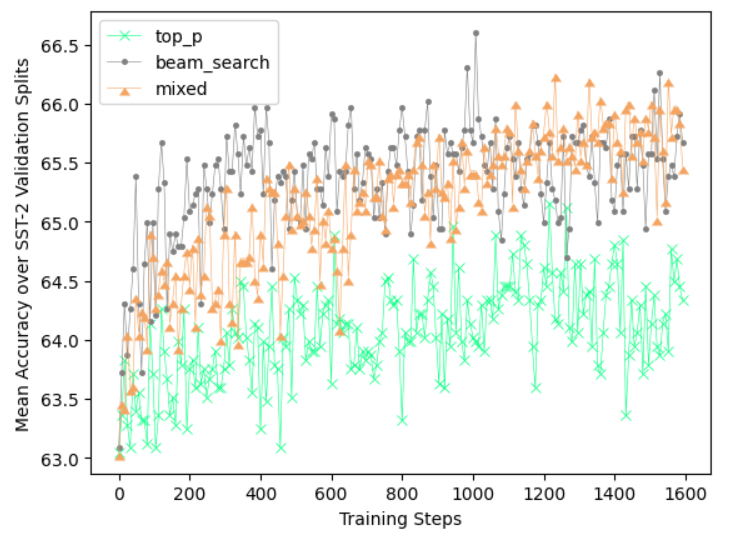
\includegraphics[width=0.7\linewidth]{decoding_in_mml.png}
    \end{figure}
\end{itemize}
\end{frame}

\begin{frame}{Decoding Techniques for PG}
\begin{itemize}
        \item - Average performance on 5 validation splits for three text decoding techniques under 128-shot training.
        \medskip
        \medskip
        \item - Further Averaging over on-policy and off-policy learning!
        \medskip
        \medskip
        \item - {\color{green}Top-p decoding} is better in PG!
        \begin{figure}
        \centering
        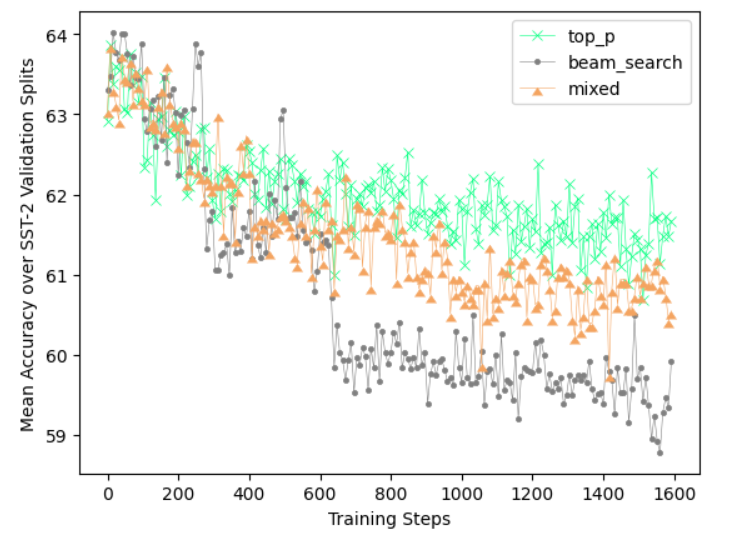
\includegraphics[width=0.7\linewidth]{decoding_in_pg.png}
    \end{figure}
\end{itemize}
\end{frame}

\begin{frame}{MML vs. PG}
\begin{itemize}
        \item - Average performance on 5 validation splits under 128-shot training.
        \medskip
        \medskip
        \item - Off-policy MML with beam-search wins!
        \begin{figure}
        \centering
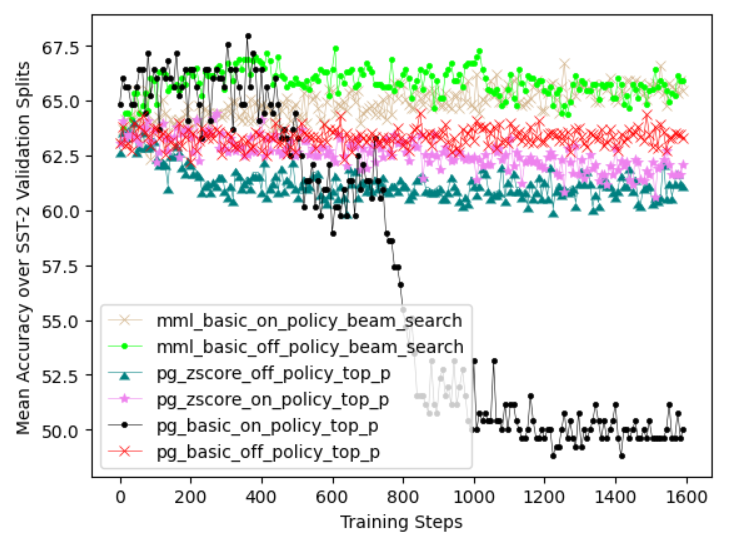
\includegraphics[width=0.7\linewidth]{comparison.png}
    \end{figure}
\end{itemize}
\end{frame}

\begin{frame}{Zero-shot Predictions after Finetuning $P_{\theta_{\text{par}}}$}
\begin{itemize}
        \item Only Averaged over paraphrases: 75.2\%\\
        \item Only Averaged over paraphrases {\color{green}after Finetuning $P_{\theta_{\text{par}}}$: 77.5\%}\\
        \medskip
        \medskip
        \medskip
        \item Averaged over paraphrases + original input: 83.3\%\\
        \item Averaged over paraphrases + original input {\color{green}after Finetuning $P_{\theta_{\text{par}}}$: 83.5\%}
\end{itemize}
\end{frame}

\bibliography{anthology,custom}
\bibliographystyle{acl_natbib}

\end{document}